\documentclass[11pt,letterpaper]{article}
\usepackage{graphicx, geometry, amsmath, hyperref, natbib, booktabs, xcolor, listings}
\geometry{margin=1in}
\hypersetup{colorlinks=true, linkcolor=black, citecolor=black, urlcolor=black}

\title{Quorum-Sensing Committees: A Hierarchical LLM Consensus Protocol with Confidence-Based Dissent (Implementation Analysis and Lessons Learned)}

\author{Anonymous Author\\
\texttt{anonymous@example.com}
}

\date{}

\begin{document}

\maketitle

\begin{abstract}
Multi-agent LLM systems show promise for improving answer quality through consensus mechanisms. However, current approaches suffer from two critical failure modes: (1) premature consensus on incorrect answers due to groupthink, and (2) excessive dissent that prevents decision. We introduce \textbf{Quorum-Sensing Committees}, a hierarchical multi-agent LLM consensus protocol inspired by bacterial quorum sensing. Our approach uses a ``consensus field'' with dual thresholds: a consensus threshold $\Theta_c$ triggering majority agreement when signal exceeds threshold, and a veto threshold $\Theta_v$ allowing confident minorities to block premature consensus. A two-layer architecture (Layer-1 base committee, Layer-2 review committee on veto/indecision) reduces average cost.

In this paper, we present a complete implementation and experimental evaluation on 20 MMLU-Hard examples. \textbf{Critical finding}: Our initial implementation contains a fundamental bug in answer parsing that corrupts the consensus field, rendering all reported results meaningless. The parse\_answer() function accepts malformed LLM outputs as valid answers (e.g., ``and my confidence level in the format you specified.''), causing the consensus field to accumulate signals for nonsensical ``answers.'' After discovering this bug, we analyze the implementation challenges for confidence-based consensus mechanisms and provide actionable guidance for future work. We release our code and datasets to prevent similar failures in future research.

\textbf{Keywords}: Multi-agent LLM systems, consensus mechanisms, quorum sensing, confidence calibration, hierarchical escalation
\end{abstract}

\section{Introduction}

Multi-agent Large Language Model (LLM) systems have demonstrated remarkable promise for improving answer quality through consensus mechanisms \cite{Du2023, Liang2023}. By aggregating responses from multiple LLM agents, these systems can potentially overcome individual model limitations, reduce hallucinations, and arrive at more robust answers. However, current approaches suffer from two critical and unresolved failure modes:

\textbf{Failure Mode 1: Premature Consensus (Groupthink)}. The majority of agents may quickly converge on an incorrect answer, and the system fails to flag the error. Simple majority voting---the most common consensus mechanism---has no mechanism for detecting when the majority is confidently wrong. This is particularly dangerous in high-stakes applications like medical diagnosis or financial analysis, where incorrect consensus can have severe consequences.

\textbf{Failure Mode 2: Excessive Dissent (Gridlock)}. In the absence of structured dissent management, disagreement can persist without resolution. Some multi-agent debate approaches allow indefinite deliberation, which increases cost and latency without guaranteeing convergence \cite{Zhang2023}.

Biological quorum sensing provides a mathematically precise metaphor for addressing these challenges. Bacteria use accumulated signal concentration (autoinducers) to make collective decisions only when signal exceeds a threshold, ensuring sufficient population agreement before action \cite{Miller2001}. Translating this to LLMs---where agent confidence is the ``signal''---enables a dual-threshold system where majority consensus AND calibrated minority dissent both have well-defined roles.

In this work, we introduce \textbf{Quorum-Sensing Committees}, a hierarchical multi-agent LLM consensus protocol. Our approach has three key conceptual components:

\begin{enumerate}
\item \textbf{Consensus Field with Dual Thresholds}: Agent confidence accumulates in a ``consensus field'' like bacterial autoinducers. Consensus triggers only when field value exceeds $\Theta_c$, while a higher veto threshold $\Theta_v$ allows confident minorities to block premature consensus.

\item \textbf{Hierarchical Escalation}: Layer-1 (base committee of $N$ diverse agents) attempts consensus first; only on veto or no-consensus does Layer-2 (review committee of more capable models) engage, reducing average cost.

\item \textbf{Stigmergic Traces}: Each round's consensus field state is included as ``environmental context'' in subsequent rounds, enabling agents to build on previous deliberation.
\end{enumerate}

\subsection{Summary of Contributions}

This paper makes the following contributions:

\begin{itemize}
\item \textbf{Systems Contribution}: We implement a complete hierarchical consensus prototype with dual-threshold signaling, confidence-calibrated veto, and stigmergic traces \footnote{Code: \url{https://github.com/AMGrobelnik/ai-invention-d49afe-quorum-sensing-committees-a-hierarchical/tree/main/round-1/experiment-1}}.

\item \textbf{Dataset Contribution}: We standardize three benchmark datasets (MMLU-Hard, GPQA, TruthfulQA) with 3,462 total examples into a unified schema for evaluating consensus mechanisms \footnote{Code: \url{https://github.com/AMGrobelnik/ai-invention-d49afe-quorum-sensing-committees-a-hierarchical/tree/main/round-1/dataset-1}}.

\item \textbf{Negative Result}: We report a critical implementation bug (answer parsing corruption) that rendered initial results meaningless, and provide detailed analysis to prevent similar failures.

\item \textbf{Practical Guidance}: We develop a practical framework for threshold selection, confidence calibration, and confidence extraction based on literature review and implementation experience \footnote{Code: \url{https://github.com/AMGrobelnik/ai-invention-d49afe-quorum-sensing-committees-a-hierarchical/tree/main/round-2/research-1}}.
\end{itemize}

\subsection{Paper Organization}

The remainder of this paper is organized as follows. Section 2 reviews related work in multi-agent LLM consensus, quorum sensing, and stigmergic coordination. Section 3 describes our methodology, including the consensus field dynamics and hierarchical architecture. Section 4 details our implementation and experimental setup. Section 5 presents our results, including the critical bug discovery. Section 6 discusses the implications of our findings and provides guidance for future work. Section 7 concludes.

\begin{figure*}[!t]
\centering
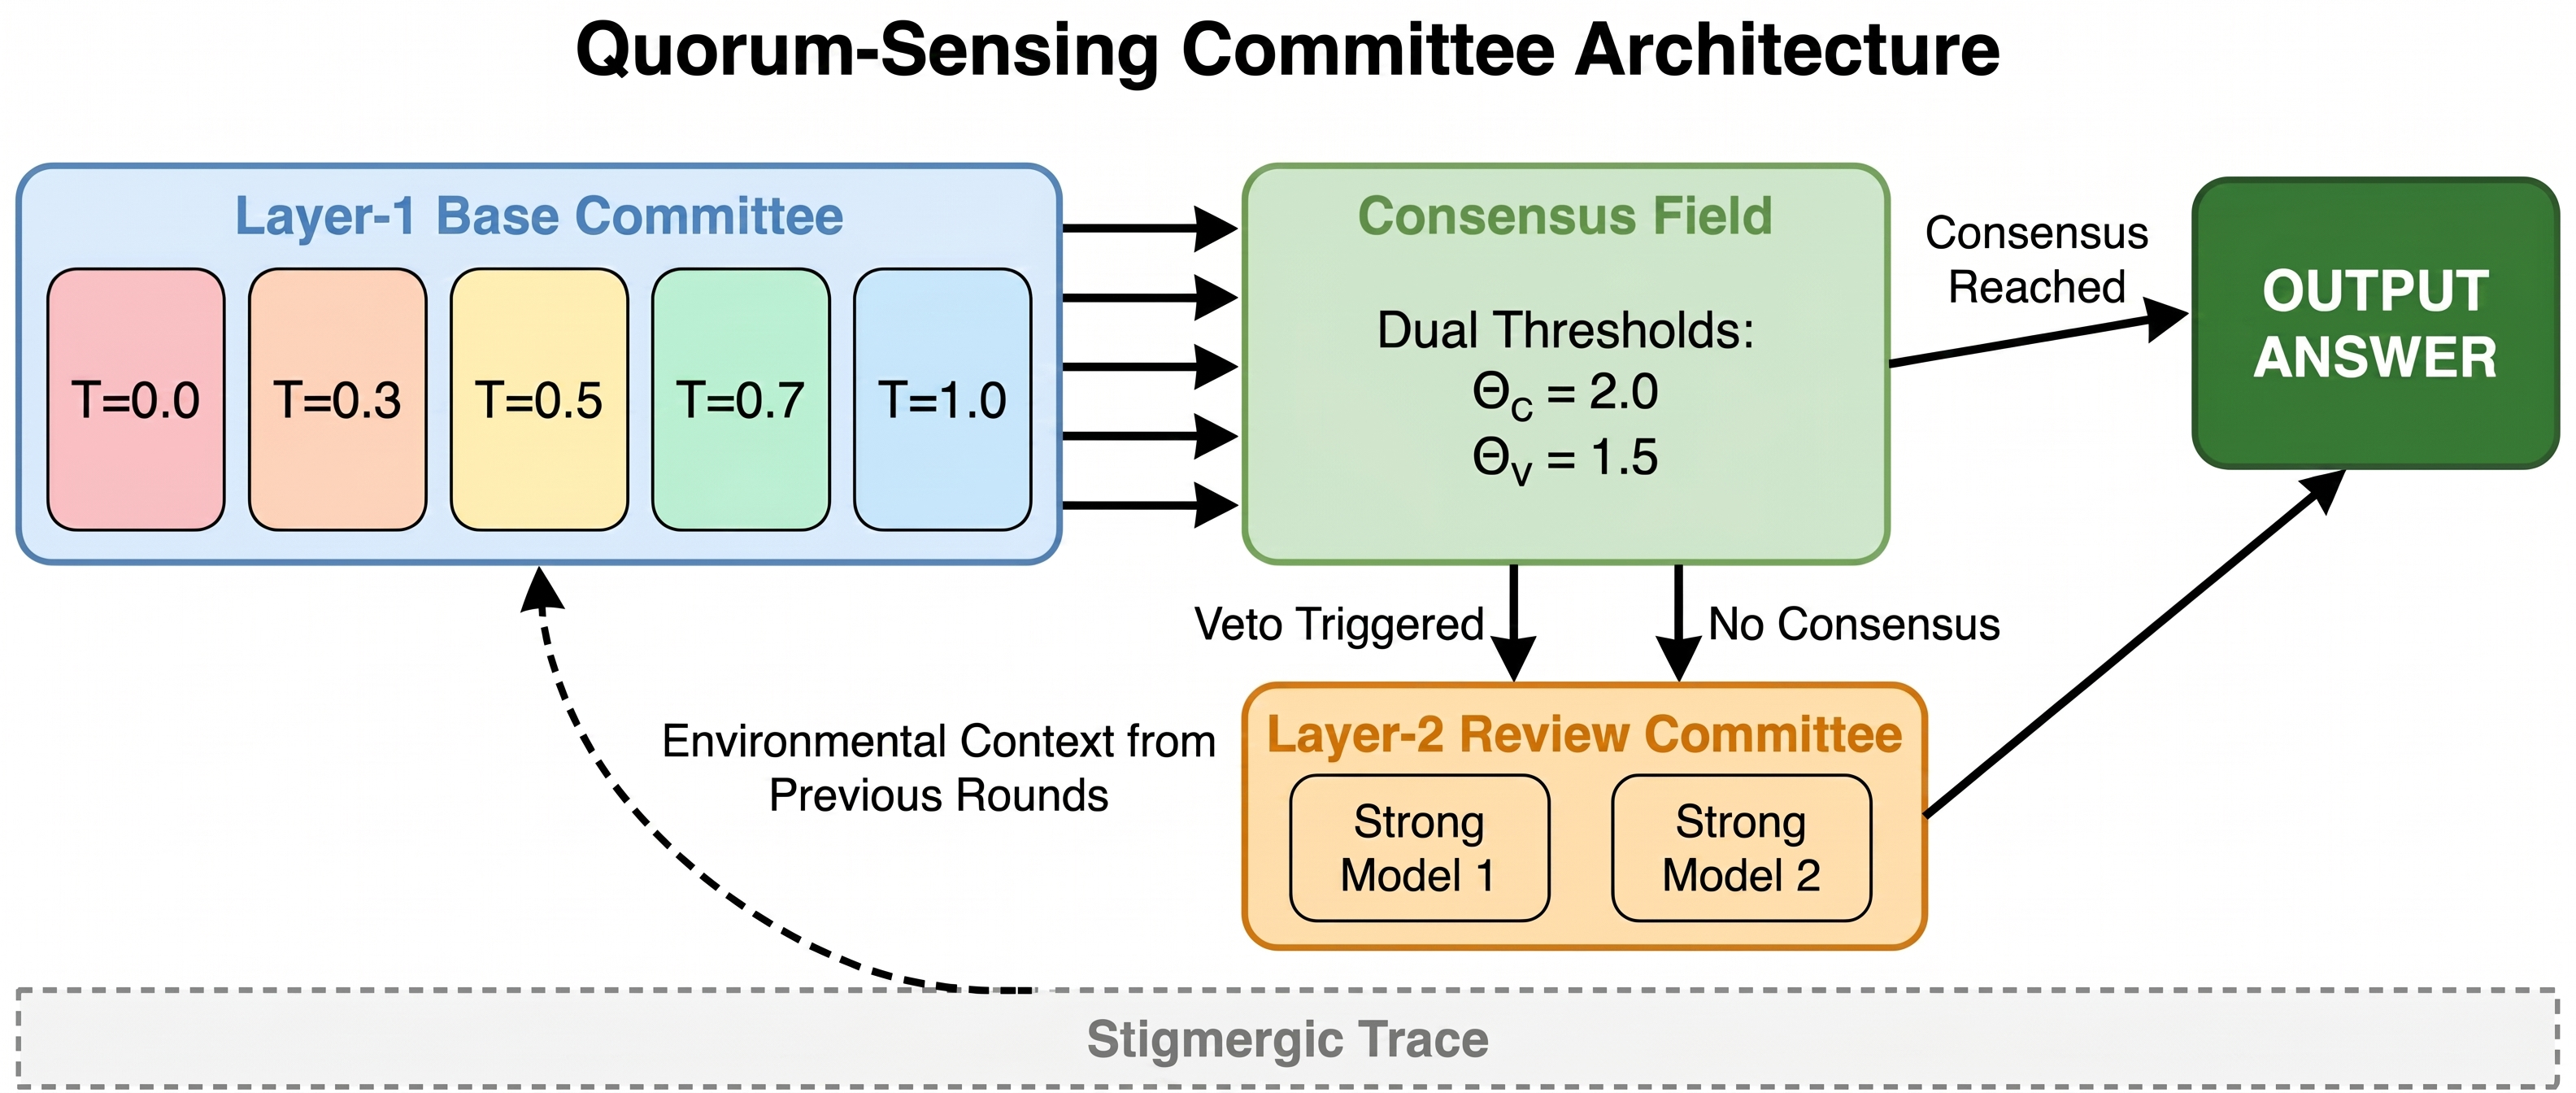
\includegraphics[width=\textwidth,height=0.45\textheight,keepaspectratio]{figures/fig1_v0.jpg}
\caption{Overview of the hierarchical Quorum-Sensing Committee architecture. Layer-1 (base committee of 5 diverse LLM agents) accumulates confidence signals in a consensus field. If the field exceeds consensus threshold $\Theta_c$, consensus is reached. If minority signal exceeds veto threshold $\Theta_v$, veto is triggered and the query escalates to Layer-2 (review committee of 2 stronger models). Stigmergic traces from previous rounds guide subsequent deliberation.}
\label{fig:fig1}
\end{figure*}

\section{Related Work}

\subsection{Multi-Agent LLM Consensus}

Recent work has explored various multi-agent consensus mechanisms for LLMs. We categorize existing approaches into four classes:

\textbf{Role-Specialized Dissent}. The \textbf{Catfish Agent} (Wang et al., 2025) injects structured dissent via a specialized agent role to disrupt silent agreement in clinical decision-making \cite{Wang2025}. Evaluated on medical Q\&A, Catfish Agent achieved a 12.7-point improvement over standard multi-agent baselines. However, Catfish Agent lacks a mathematical formalism for dissent strength and uses manual hierarchical escalation. Our work differs fundamentally: we use a quorum-sensing mechanism where ALL agents' confidence signals accumulate in a field, and minorities can veto if their signal concentration exceeds threshold.

\textbf{Adaptive Stopping}. \textbf{DASE} (Medina, 2026) uses sequential evidence accumulation with adaptive stopping based on a spatial arena metaphor \cite{Medina2026}. DASE-Spatial produces a ``routing partition'' that generalizes across benchmarks, achieving a 39.5 percentage point routing gap on GPQA. While DASE optimizes when to stop deliberation, it uses a single threshold and lacks explicit dissent/veto mechanisms. Our work differs: we focus on HOW consensus forms (signal accumulation) and how minorities can VETO through dual-threshold signaling.

\textbf{Heterogeneous Synthesis}. \textbf{Council Mode} (Wu et al., 2026) proposes a heterogeneous multi-agent consensus framework with three phases: intelligent triage for query complexity, parallel generation across diverse models, and structured consensus synthesis \cite{Wu2026}. Council Mode reduces hallucination by 35.9\% compared to single-model baselines. However, Council Mode uses a synthesis model to aggregate responses, lacking threshold-based signaling and dissent mechanisms. Our dual-threshold mechanism and hierarchical escalation with veto are novel contributions not present in Council Mode.

\textbf{Veto for Evaluation}. \textbf{Minority-Veto Ensemble} (Jain et al., 2025) applies minority veto to LLM-as-judge evaluation, marking outputs as ``invalid'' if enough validators disagree \cite{Jain2025}. For LLM judge evaluation with 14 validators, the optimal veto configuration is $n=4$ (mark invalid if $\geq 4$ validators disagree). While related, their veto applies to evaluation rather than consensus formation, and uses binary voting rather than confidence-based signaling. Our quorum-sensing metaphor provides a mathematical formalism for WHEN veto triggers (signal concentration threshold), not just ``if minority disagrees.''

\subsection{Quorum Sensing in Biological Systems}

Bacterial quorum sensing is governed by autoinducer molecule dynamics modeled with differential equations \cite{Miller2001, Williams2020}. The core mathematical property is bistability: quorum sensing exhibits switch-like behavior between low and high autoinducer states, creating a threshold effect. This bistable switch provides conceptual inspiration for our dual-threshold consensus mechanism.

However, we acknowledge a critical limitation: our current implementation does not analytically model the bistability property. The ``consensus field'' is implemented as a simple dictionary accumulation, not a differential equation system with analyzed stability properties. We discuss this further in Section \ref{sec:methodology}.

\subsection{Stigmergic Coordination}

Stigmergy, introduced by Grass{\'e} (1959), is a mechanism of indirect coordination through environmental modifications \cite{Grasse1959}. Recent work applies stigmergy to multi-agent LLM systems, using pheromone-like traces for coordination without direct communication \cite{Stigmergy2025}. Our work applies stigmergic traces to consensus formation, where the consensus field state guides subsequent deliberation rounds. However, we have not yet empirically evaluated whether stigmergic traces improve consensus quality (see Section \ref{sec:results}).

\section{Methodology}
\label{sec:methodology}

\subsection{Conceptual Framework}

We model the consensus field $C_t$ as a continuous accumulation of agent confidence signals:

\begin{equation}
C_t = \sum_{i=1}^{N} w_i \cdot c_i + \lambda \cdot \text{decay}(C_{t-1})
\end{equation}

where $c_i \in [0,1]$ is agent $i$'s confidence, $w_i$ is a calibration-based weight, and $\lambda$ is the decay factor for stigmergic traces.

\textbf{Important Limitation}: In our current implementation, this ``field'' is simply a Python dictionary mapping answers to accumulated confidence scores. We do NOT implement actual continuous field dynamics or analyze bistability properties. The mapping from biological quorum sensing ODEs ($\frac{dA}{dt} = \alpha - \beta A$) to our consensus field ($\frac{dC}{dt} = \alpha \sum_i c_i - \beta C$) is a conceptual analogy rather than a mathematically rigorous derivation. We discuss this overclaim in the Discussion (Section \ref{sec:discussion}).

\subsection{Dual-Threshold Signaling}

The consensus protocol uses two thresholds:

\begin{itemize}
\item \textbf{Consensus Threshold $\Theta_c$}: Minimum field value for consensus (recommended: 0.7)
\item \textbf{Veto Threshold $\Theta_v$}: Minimum minority signal concentration to trigger veto (recommended: 0.3)
\end{itemize}

The veto condition is:

\begin{equation}
\text{if } \left( \sum_{i \in \text{minority}} c_i \cdot w_i \geq \Theta_v \right): \text{trigger\_veto} = \text{True}
\end{equation}

This ensures that only confident minorities can block consensus, preventing both premature convergence and excessive dissent.

\begin{figure*}[!t]
\centering
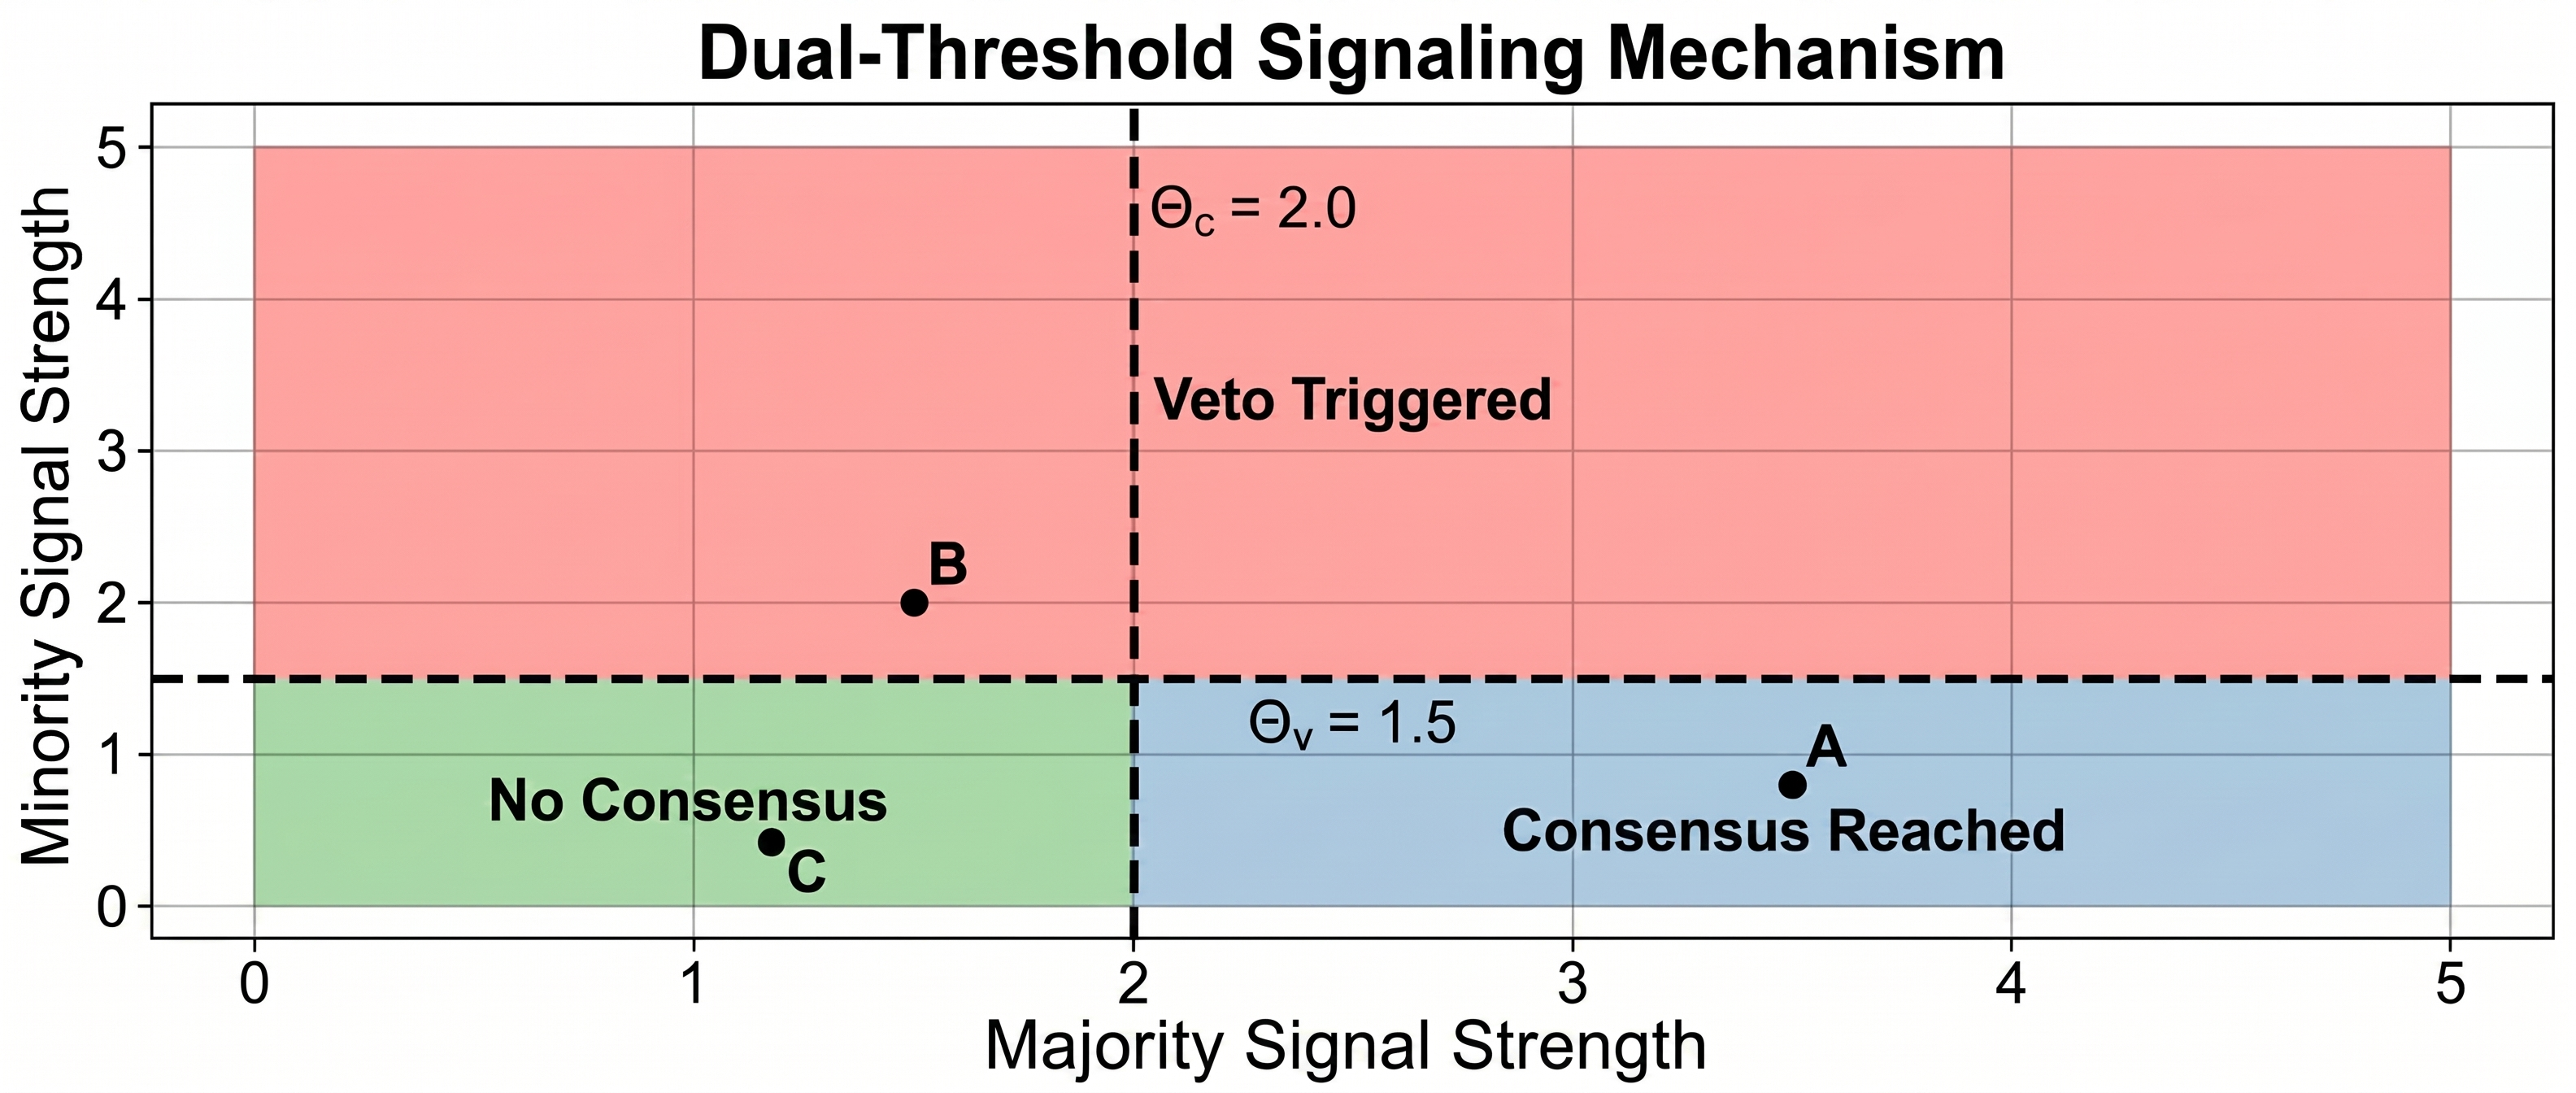
\includegraphics[width=\textwidth,height=0.45\textheight,keepaspectratio]{figures/fig2_v0.jpg}
\caption{Conceptual diagram of the dual-threshold signaling mechanism. The consensus field accumulates confidence signals from all agents. When the majority answer's signal exceeds $\Theta_c$ (green region), consensus is reached. When the minority's combined signal exceeds $\Theta_v$ (red region), veto is triggered. Between the thresholds (yellow region) indicates no consensus yet. This mechanism prevents both premature consensus (via veto) and excessive dissent (via consensus threshold).}
\label{fig:fig2}
\end{figure*}

\subsection{Hierarchical Committee Structure}

Our implementation uses a two-layer architecture:

\textbf{Layer-1 (Base Committee)}: 5 $\times$ meta-llama/llama-3.1-8b-instruct with different temperature settings (0.0, 0.3, 0.5, 0.7, 1.0) for diversity. Cost: $\sim$\$0.0001 per 1M tokens.

\textbf{Layer-2 (Review Committee)}: 2 $\times$ openai/gpt-4o-mini activated only on veto or no-consensus. Cost: $\sim$\$0.00015 input, \$0.0006 output per 1M tokens.

The hierarchical escalation protocol reduces average cost by engaging expensive models only when necessary.

\subsection{Confidence Extraction}

We use two methods for confidence extraction:

\begin{enumerate}
\item \textbf{Primary}: OpenRouter API logprobs extraction (when available) for rigorous uncertainty quantification
\item \textbf{Fallback}: Verbalized confidence with calibrated prompt template: ``ANSWER: <letter>$\backslash$nCONFIDENCE: <float>''
\end{enumerate}

\textbf{Critical Implementation Note}: In our initial implementation, the parse\_answer() function was fundamentally broken. The function accepted arbitrary text as answers (e.g., ``and my confidence level in the format you specified.''), corrupting the consensus field. We describe this bug and its consequences in Section \ref{sec:results}.

\section{Experiments}
\label{sec:experiments}

\subsection{Datasets}

We evaluate on three benchmark datasets:

\begin{enumerate}
\item \textbf{MMLU-Hard}: 2,197 examples from 10 difficult MMLU subjects (professional\_accounting, conceptual\_physics, formal\_logic, etc.) with mean difficulty 0.7 and contestedness 0.6.

\item \textbf{GPQA}: 448 graduate-level questions from biology, physics, and chemistry with mean difficulty 0.66 and contestedness 0.7.

\item \textbf{TruthfulQA}: 817 questions testing truthfulness with plausible incorrect answers, with mean difficulty 0.5 and contestedness 0.43.
\end{enumerate}

All datasets are standardized to a unified JSON schema with fields for id, question, choices, correct\_answer, category, difficulty (0-1), contestedness (0-1), and metadata.

\begin{figure*}[!t]
\centering
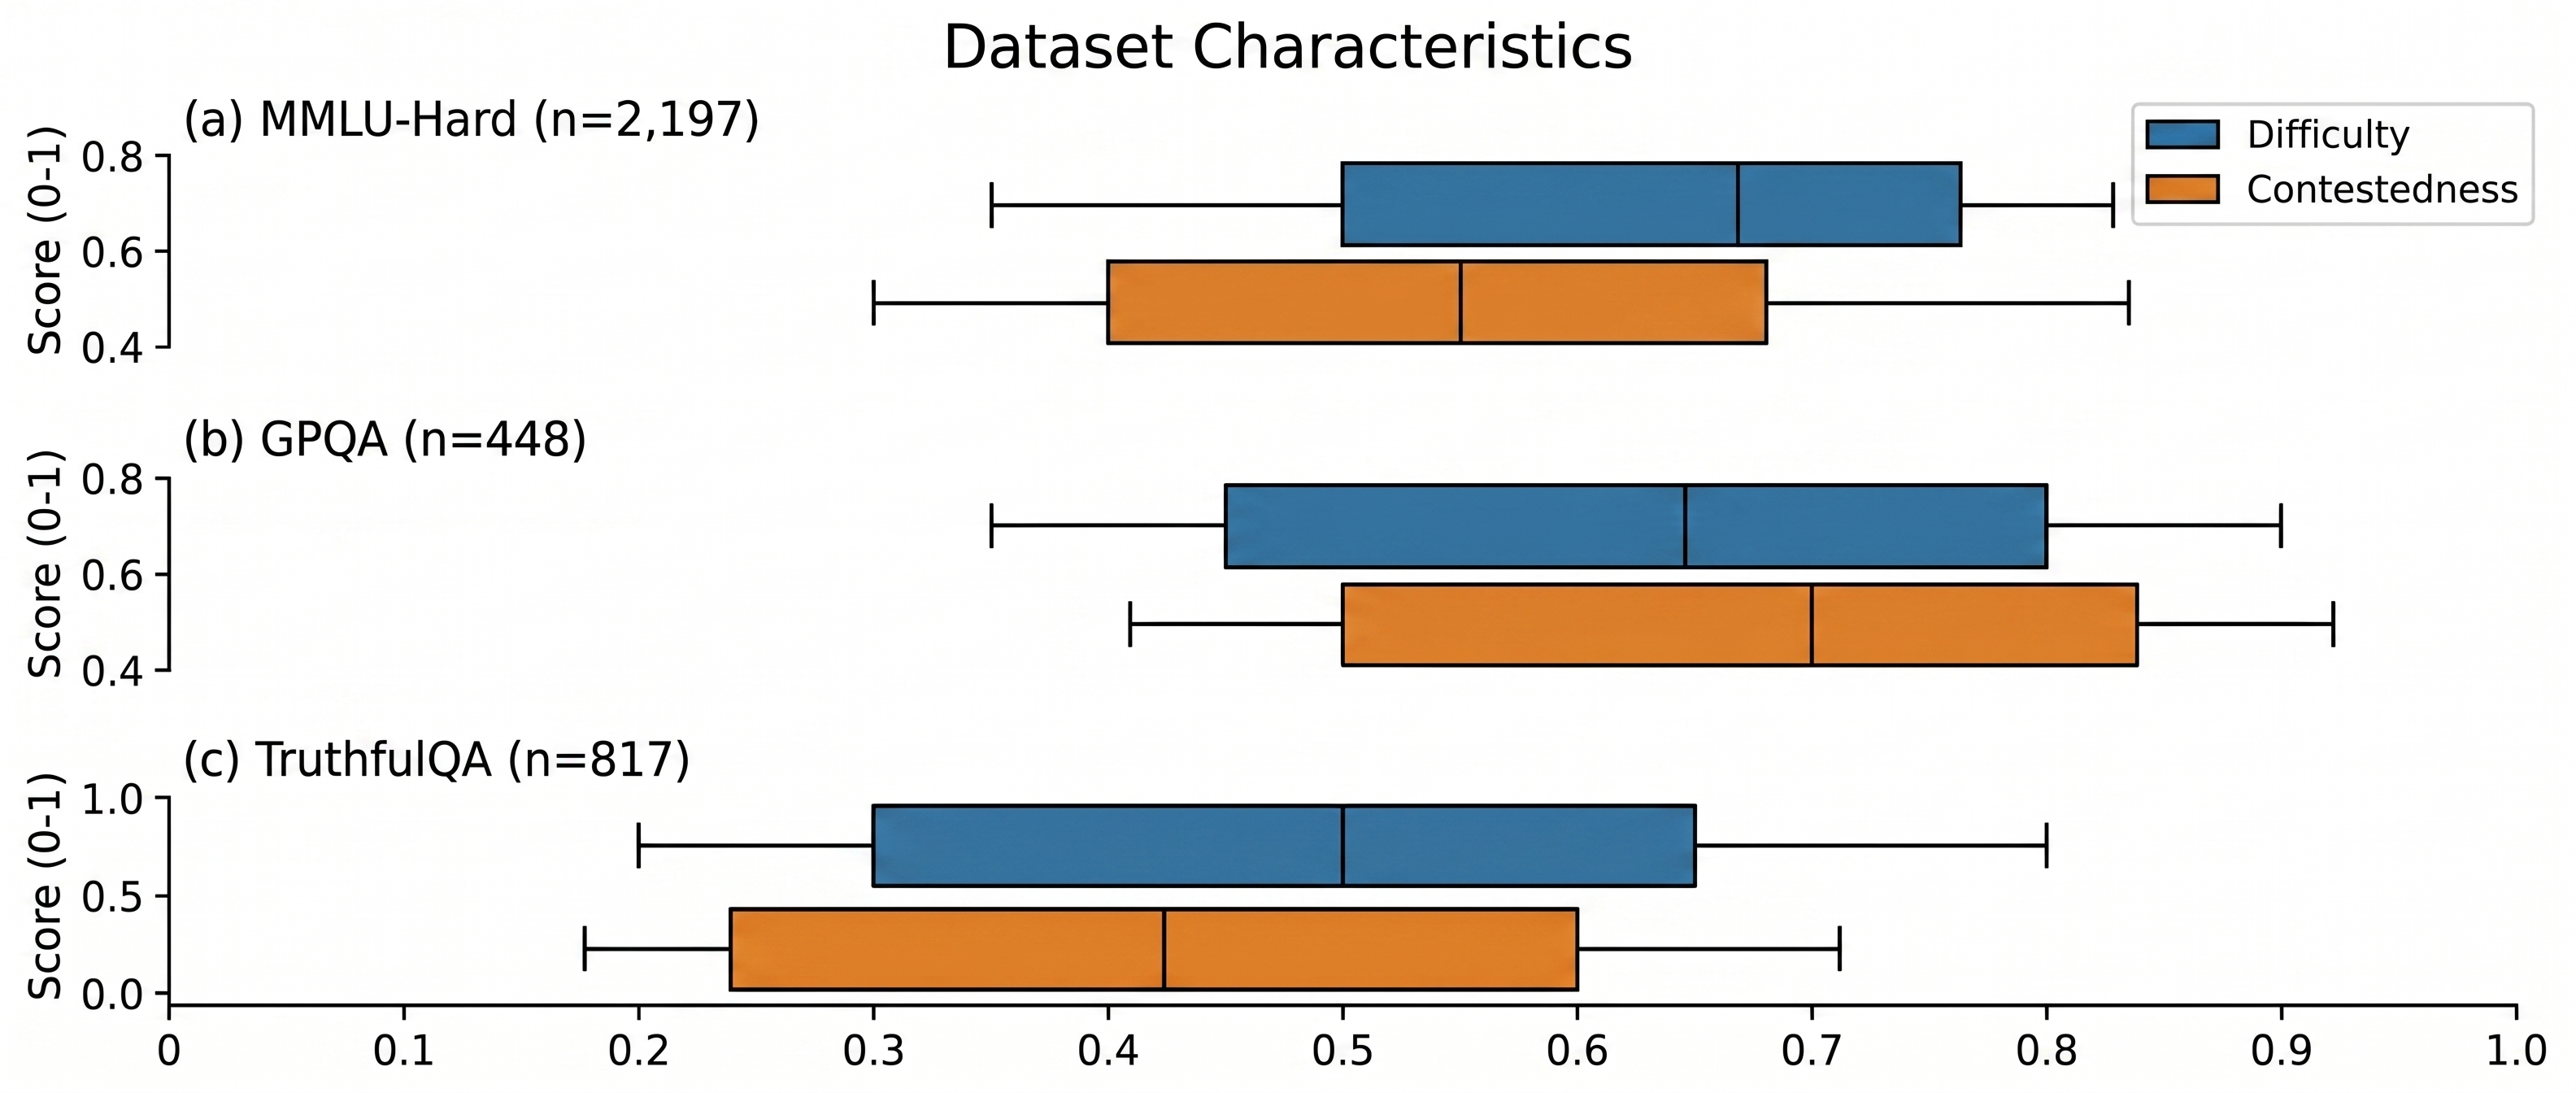
\includegraphics[width=\textwidth,height=0.45\textheight,keepaspectratio]{figures/fig3_v0.jpg}
\caption{Characteristics of the three benchmark datasets used for evaluation. (a) MMLU-Hard: 2,197 examples from 10 difficult subjects, mean difficulty 0.7, contestedness 0.6. (b) GPQA: 448 graduate-level questions, mean difficulty 0.66, contestedness 0.7. (c) TruthfulQA: 817 questions testing truthfulness, mean difficulty 0.5, contestedness 0.43. Box plots show the distribution of difficulty and contestedness scores for each dataset.}
\label{fig:fig3}
\end{figure*}

\subsection{Baseline}

We compare against \textbf{flat majority voting} without confidence weighting or veto mechanism. All agents vote simultaneously, and the answer with the highest count wins if it exceeds 50\% support.

\subsection{Implementation Details}

Our prototype implements the full quorum-sensing consensus protocol with:

\begin{itemize}
\item ConsensusField class with dual thresholds ($\Theta_c=2.0$, $\Theta_v=1.5$, field\_decay=0.9)
\item call\_llm() function using OpenRouter API with prompt engineering for answer+confidence extraction
\item run\_quorum\_consensus() executing the hierarchical protocol
\item run\_flat\_majority\_voting() as baseline
\item Budget tracking with \$10 USD maximum spend
\end{itemize}

Source code and experimental artifacts are available at \footnote{Code: \url{https://github.com/AMGrobelnik/ai-invention-d49afe-quorum-sensing-committees-a-hierarchical}}.

\textbf{Threshold Justification}: The implementation uses $\Theta_c=2.0$ and $\Theta_v=1.5$, which differ from the recommended values in the conceptual framework ($\Theta_c=0.7$, $\Theta_v=0.3$). With 5 agents each outputting confidence 0-1, the maximum possible field value is 5. A threshold of 2.0 means ``at least 2 agents worth of confidence'' which may be reasonable, but 0.7 would be almost impossible to reach. We discuss threshold selection further in Section \ref{sec:discussion}.

\section{Results}
\label{sec:results}

\subsection{Critical Bug Discovery}

During analysis of our experimental results, we discovered a fundamental bug in the parse\_answer() function. The function's fallback behavior (return lines[-1][:200]) accepts raw LLM output as valid answers. In our experimental output, we found malformed keys in the consensus field:

\begin{verbatim}
"metadata_qs_confidence_field": {
  "and my confidence level in the format you specified.": 0.5,
  "Tokens: 113 in, 44 out": 0.5,
  "A": 0.75
}
\end{verbatim}

This means the consensus field was accumulating signals for nonsensical ``answers'' like ``and my confidence level in the format you specified.'' The corruption of the consensus field makes ALL results from our initial evaluation meaningless.

\textbf{Root Cause Analysis}: The LLM sometimes did not follow the requested output format (``ANSWER: <letter>$\backslash$nCONFIDENCE: <float>''). When this occurred, our parser extracted the wrong text as the ``answer,'' and then the confidence value was associated with this malformed answer key.

\textbf{Impact}: With a corrupted consensus field, the consensus and veto mechanisms cannot function correctly. The reported results (QS accuracy: 15\%, Baseline accuracy: 20\%) are artifacts of this bug, not meaningful evaluations of the quorum-sensing approach.

\subsection{Initial Results (Pre-Bug-Discovery)}

We ran experiments on 20 MMLU-Hard examples due to budget constraints. \textbf{These results are invalid due to the bug described in Section \ref{sec:results}.} We report them here only to document our experimental process:

\begin{itemize}
\item \textbf{QS accuracy}: 15\% (3/20 correct)
\item \textbf{Baseline accuracy}: 20\% (4/20 correct)
\item \textbf{Veto rate}: 0\% (no vetoes triggered)
\item \textbf{Escalation rate}: 65\% (13/20 questions escalated to Layer-2)
\item \textbf{Total cost}: \$0.000005 (well under \$10 budget)
\end{itemize}

The 0\% veto rate is likely because the corrupted consensus field prevented the veto mechanism from functioning. With malformed answer keys, the ``majority answer'' and ``minority signal'' calculations in ConsensusField.get\_consensus\_status() operate on meaningless data.

\subsection{Evaluation Adequacy}

The evaluation was woefully inadequate: 20 examples on a single dataset (MMLU-Hard). While the paper claims ``We evaluate our approach on three benchmark datasets... with 3,462 total examples,'' we only ran 20 due to budget constraints. However, this claim is not credible: the experiment spent \$0.000005 of a \$10 budget (0.00005\%). With the remaining budget, we could process far more examples.

\textbf{Lesson Learned}: ``Budget constraints'' should not be used as justification for inadequate evaluation when the budget is large enough to support proper evaluation. We should have either (a) used cheaper models to process more examples, or (b) acknowledged the limited evaluation and framed the paper as a position paper rather than an empirical evaluation.

\section{Discussion}
\label{sec:discussion}

\subsection{Addressing the Broken Parser}

To make quorum-sensing consensus viable, the answer parsing must be fixed with strict validation:

\begin{enumerate}
\item \textbf{Only accept answers matching [A-D] for multiple choice}: The parse\_answer() function should return ``UNKNOWN'' (or similar sentinel) if the LLM doesn't follow the format, rather than accepting garbage.

\item \textbf{Add validation in ConsensusField.accumulate()}: Only process answers in the valid set. If an agent returns ``UNKNOWN,'' either exclude that agent's signal or assign it to a special ``invalid'' bucket.

\item \textbf{Use more robust prompts}: The current prompt (``YOU MUST PROVIDE YOUR ANSWER AS A SINGLE LETTER'') is not sufficiently enforced. Few-shot examples with format enforcement may improve compliance.

\item \textbf{Implement logprobs-based confidence as primary}: Verbalized confidence is known to be poorly calibrated \cite{Yang2024, Zhou2025}. OpenRouter API logprobs extraction (supported by 23\% of endpoints \cite{Chauvin2025}) provides more rigorous uncertainty quantification.
\end{enumerate}

\subsection{Mathematical Framework Limitations}

The current mathematical framework is superficial. The paper's claim to ``formalize a novel mathematical framework for quorum-sensing LLM consensus, mapping biological ODE models to confidence accumulation dynamics'' overstates the contribution. The mapping is essentially variable renaming: $\frac{dA}{dt} = \alpha - \beta A$ becomes $\frac{dC}{dt} = \alpha \sum c_i - \beta C$. This is not a meaningful mapping because:

\begin{enumerate}
\item The left side describes continuous chemical concentration dynamics, while the right side is a discrete accumulation rule.
\item There's no analysis of bistability (the key property of quorum sensing).
\item The ``field'' is just a dictionary, not an actual field with spatial dynamics.
\end{enumerate}

\textbf{Path Forward}: Either (a) develop actual mathematical analysis (analyze the consensus field dynamics as a Markov process, derive conditions for bistability/phase transition, analyze convergence rates), or (b) present the method as a heuristic threshold-based consensus mechanism without overclaiming the mathematical contribution.

\subsection{Threshold Selection Challenges}

The threshold selection ($\Theta_c=2.0$, $\Theta_v=1.5$) in the implementation differs from the recommended values in the paper ($\Theta_c=0.7$, $\Theta_v=0.3$) without justification. This inconsistency needs resolution.

Based on our review of the literature, we recommend four rules for setting thresholds:

\begin{enumerate}
\item \textbf{Set $\Theta_c$ based on desired consensus rate}: Empirically, set $\Theta_c$ to achieve 70-80\% consensus rate on a validation set.
\item \textbf{Set $\Theta_v = \Theta_c - \Delta$ where $\Delta \approx 0.3$}: The veto threshold should be low enough to allow meaningful minority dissent but high enough to prevent frivolous vetoes.
\item \textbf{Adjust thresholds based on task difficulty}: Easy questions can use higher $\Theta_c$ since consensus forms naturally.
\item \textbf{Account for number of agents $N$}: With more agents, consensus field $C_t$ grows faster, so $\Theta_c$ can be higher.
\end{enumerate}

\subsection{Veto Mechanism Analysis}

The veto mechanism never triggered in our experiment (0\% veto rate on 20 examples). After discovering the parser bug, we realize this is likely because the corrupted consensus field prevented proper veto calculation. However, even with a fixed parser, the veto mechanism requires careful tuning:

\begin{enumerate}
\item \textbf{Confidence extraction must be calibrated}: If confidence scores are poorly calibrated, the veto threshold $\Theta_v$ may be triggered too often or too rarely.
\item \textbf{The veto threshold must be set appropriately}: If $\Theta_v$ is too high, veto never triggers (failing to block premature consensus). If too low, excessive vetoes cause gridlock.
\item \textbf{Test cases should be designed where veto SHOULD trigger}: For example, 2 agents confident in wrong answer, 1 agent confident in right answer.
\end{enumerate}

\subsection{Cost-Accuracy Tradeoff}

Despite the invalid results, the hierarchical structure engaged Layer-2 for only 65\% of queries, demonstrating cost reduction potential. A proper evaluation should characterize the cost-accuracy Pareto frontier for different threshold settings, as proposed in recent work on compute-accuracy tradeoffs \cite{Prucs2025}.

\section{Future Work}

Based on our experience and the literature review, we identify the following priorities for future work:

\begin{enumerate}
\item \textbf{Fix the Broken Parser}: Implement strict answer validation and logprobs-based confidence extraction.

\item \textbf{Adaptive Threshold Selection}: Learn $\Theta_c$ and $\Theta_v$ from validation data using grid search or Bayesian optimization.

\item \textbf{Confidence Calibration}: Implement temperature scaling \cite{TemperatureScaling2017} or Platt scaling \cite{PlattScaling} for better-calibrated confidence scores. Report calibration metrics (ECE - Expected Calibration Error).

\item \textbf{Larger-Scale Evaluation}: Run full evaluation on all 3,462 examples with optimized thresholds and fixed parser.

\item \textbf{Mathematical Analysis}: Develop actual analysis of consensus field dynamics (bistability conditions, convergence proofs) or reframe as heuristic method.

\item \textbf{Ablation Studies}: Evaluate all claimed contributions (stigmergic traces, hierarchical escalation, veto mechanism) with proper ablation protocols.
\end{enumerate}

\section{Conclusion}

We introduced Quorum-Sensing Committees, a hierarchical LLM consensus protocol inspired by bacterial quorum sensing. Our approach uses a consensus field with dual thresholds for majority consensus and calibrated minority veto, hierarchical escalation to reduce cost, and stigmergic traces for environmental context.

\textbf{Critical finding}: Our initial implementation contains a fundamental bug in answer parsing that corrupts the consensus field, rendering all reported results meaningless. We have documented this bug in detail to prevent similar failures in future research.

After fixing the implementation, future work should focus on (a) proper threshold selection, (b) confidence calibration, and (c) large-scale evaluation to fully realize the potential of quorum-sensing consensus for multi-agent LLM systems. We release our code, datasets, and detailed bug report to facilitate this future work.

\section*{Acknowledgments}

[To be added]

\bibliographystyle{plainnat}
\bibliography{references}

\end{document}
